\documentclass[12pt]{article}
\usepackage{Shapes}
\usepackage[utf8]{vietnam}
\usepackage{microtype}
\usepackage{mathtools,amssymb}
\usepackage{diagbox}
\usepackage{lmodern}
\usepackage{listings}
\usepackage{tikz}
\usepackage{tasks}
\usepackage{xcolor}
\usepackage{hyperref}
\usepackage{caption}
\usepackage{float}
%%%%%%%%%%%%
% \usepackage{indentfirst}
\setlength{\parindent}{0pt}
\usepackage{tikz}
\usepackage{pgfplots}
\usetikzlibrary{shapes.geometric, arrows}
\newcounter{example}[section]
\newenvironment{example}[1][]{\refstepcounter{example}\medskip
   \textbf{Ví dụ~\theexample : #1} \rmfamily}{\medskip}

\newcounter{defs}[subsection]
\newenvironment{defs}[1][]{\refstepcounter{defs}
   \textbf{Định nghĩa~\thesubsection.\thedefs : #1} \rmfamily}

\newcounter{clause}[subsection]
\newenvironment{clause}[1][]{\refstepcounter{clause}\medskip
   \textbf{Mệnh đề~\thesubsection.\theclause : #1} \rmfamily}{\medskip}
%%%%%%%%%%%%%%%%%%%

\usepackage{titlesec}
\usepackage{mdframed}

\usepackage{relsize}

\usepackage{mathptmx}
\usepackage{amsthm}
\usepackage{multicol}

\theoremstyle{definition}
\newtheorem{definition}{Định nghĩa}[section]

\theoremstyle{definition}
\newtheorem{theorem}{Định lý}[section]

\newtheorem*{remark}{Nhận xét}

\newtheorem{vd}{Ví dụ}[section]
\newtheorem{bt}{Bài tập}[section]
\newtheorem{tc}{Tính chất}[section]
\newtheorem{md}{Mệnh đề}[section]
\newtheorem{cy}{Chú ý}[section]
%%%%%%%%%%%%%%%%%%%


%\fancyhead[LO, RE]{Toán Tin 01 - k64}
%\fancyhead[LE, RO, font=\bfseries, color=HustRed]{MI4024 - Lớp 129852}
\definecolor{dkgreen}{rgb}{0,0.6,0}
\definecolor{Gray}{rgb}{0.5,0.5,0.5}
\definecolor{mauve}{rgb}{0.58,0,0.82}
\definecolor{cadmiumorange}{rgb}{0.93, 0.53, 0.18}
\definecolor{sami}{RGB}{1,90,143}
\lstdefinestyle{mystyle}{
	frame=shadowbox,
  language=SQL,
  aboveskip=3mm,
  belowskip=3mm,
  showstringspaces=false,
  columns=flexible,
  basicstyle={\normalsize\ttfamily},
  numbers=left,
  numberblanklines=true,
  numbersep=5pt,
  numberstyle=\tiny\color{gray},
  keywordstyle=\color{sami},
  morekeywords={USE},
  commentstyle=\color{dkgreen},
  stringstyle=\color{cadmiumorange},
  breaklines=true,
  breakatwhitespace=true,
  tabsize=2,
  keepspaces=true
}
\lstset{style=mystyle}
\title{\begin{center}
    Mô phỏng khung cảnh của một ngôi nhà
\end{center}}
\subtitle{\begin{center}
    LẬP TRÌNH 3D
\end{center}%\\Chủ đề:\\ SMS Spam - Xử lý tin nhắn Spam 
}
\author{
Nhóm sinh viên thực hiện: & Nhóm 1\\
Lê Thanh Thảo & 20195919\\
Phạm Thu Trang & 20195931\\[0.5cm]
%MSSV: & 20195931\\
Mã lớp: & 137976\\
Mã học phần: & MI4332\\
Học kỳ: & 20221
}
\info{\textbf{Giảng viên hướng dẫn: Vương Mai Phương} 
}
\logo[scale=0.62]{logotitle.png}
\definecolor{codegreen}{rgb}{0,0.6,0}
\definecolor{codegray}{rgb}{0.5,0.5,0.5}
\definecolor{codepurple}{rgb}{0.58,0,0.82}
\definecolor{backcolour}{rgb}{0.95,0.95,0.92}

\lstdefinestyle{mystyle}{
    backgroundcolor=\color{backcolour},   
    commentstyle=\color{codegreen},
    keywordstyle=\color{magenta},
    numberstyle=\tiny\color{codegray},
    stringstyle=\color{codepurple},
    basicstyle=\ttfamily\footnotesize,
    breakatwhitespace=false,         
    breaklines=true,                 
    captionpos=b,                    
    keepspaces=true,                 
    numbers=left,                    
    numbersep=5pt,                  
    showspaces=false,                
    showstringspaces=false,
    showtabs=false,                  
    tabsize=2
}
\lstset{style=mystyle}


%---------------------------------------------------------------------
\newmdenv[linecolor=black,skipabove=\topsep,skipbelow=\topsep,      %|
leftmargin=-5pt,rightmargin=-5pt,                                   %|
innerleftmargin=5pt,innerrightmargin=5pt]{mybox}                    %|
%---------------------------------------------------------------------
\begin{document}
\maketitlepage
\newpage
\tableofcontents
\newpage
\listoffigures
\newpage
%\listoftables

\newpage

\addcontentsline{toc}{section}{\bfseries Mở đầu}
\section*{Mở đầu}
Trong bài báo cáo này, chúng em sẽ trình bày sản phẩm mà nhóm chúng em đã làm ra được. Đó là một sản phẩm 3D về một ngôi nhà với các khung cảnh xung quanh nó và tạo cả được một cái model là các đồ đạc chi tiết bên trong căn nhà. Chúng em rất mong nhận được góp ý của thầy và các bạn trong lớp để bài cáo được hoàn thiện hơn.\\

\indent Chúng em xin chân thành cảm ơn cô Vương Mai Phương đã luôn nhiệt tình giảng dạy, truyền đạt những kiến thức về môn Lập trình 3D để giúp chúng em có thể hoàn thiện bài báo cáo này.

\indent Chúng em xin chân thành cảm ơn!

\begin{minipage}{0.5\textwidth}
\end{minipage}
\hspace{0.5\textwidth}
\begin{minipage}{0.5\textwidth}
	\noindent\begin{center}
		\vspace{0.5cm}
		\textit{Hà Nội, tháng 2 năm 2023}
		\textbf{}
	\end{center}	
\end{minipage}

\newpage
\renewcommand{\arraystretch}{2}





\newpage 
\section{Giới thiệu sản phẩm}
Bài tập lớn của chúng em mô phỏng hai khung cảnh chính sau:
\begin{itemize}
    \item Khung cảnh ngoài trời
    \item Khung cảnh trong ngôi nhà 
\end{itemize}
\subsection{Khung cảnh ngoài trời}
Trong phần này, chúng em mô phỏng khung cảnh một ngôi nhà nằm giữa rừng cây và thêm hiệu ứng những đám mây đang trôi trên bầu trời. Khung cảnh được hiện lên trong hai thời điểm: ban ngày và ban đêm. 
\begin{center}
    \begin{figure}[!h]
        \centering
        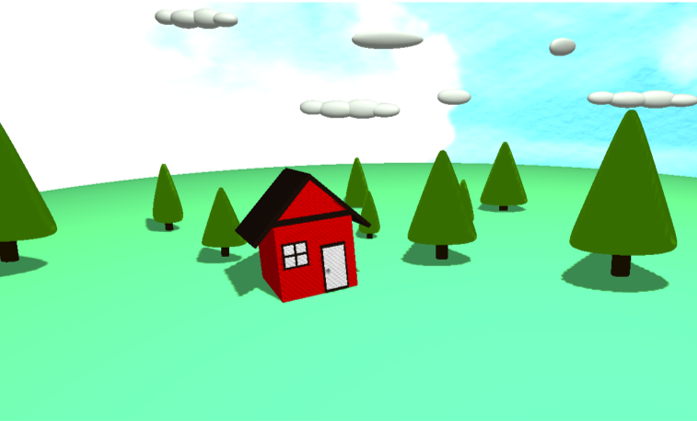
\includegraphics[scale = 0.85]{contents/out day.png}
        \caption{Khung cảnh ngoài trời vào ban ngày}
    \end{figure}
\end{center}
\newpage 
\begin{center}
    \begin{figure}[!h]
        \centering
        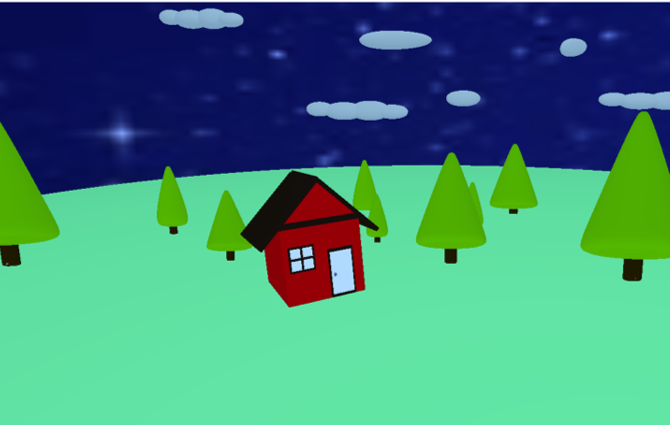
\includegraphics[scale = 0.85]{contents/outdoornight.png}
        \caption{Khung cảnh ngoài trời vào ban đêm}
    \end{figure}
\end{center}
\subsection{Khung cảnh trong ngôi nhà}
Trong phần này, chúng em mô phỏng khung cảnh bên trong ngôi nhà gồm các đối tượng: giường, tủ, bàn học, chậu cây, thảm,... Các đối tượng này được sắp xếp vào các vị trí phù hợp với nhau.
\begin{center}
    \begin{figure}[!h]
        \centering
        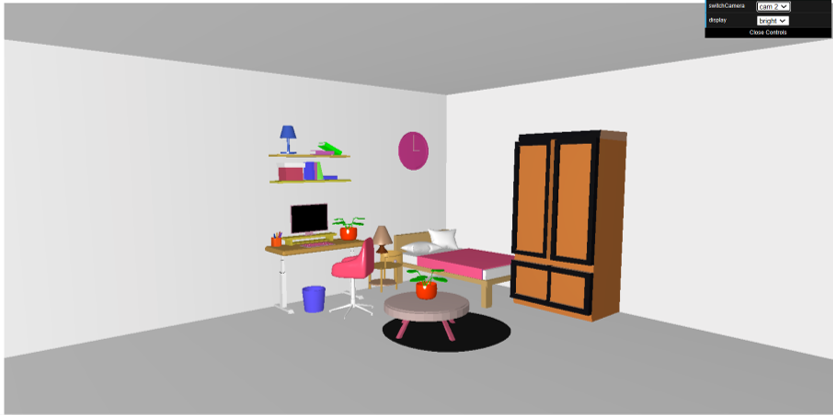
\includegraphics[scale = 0.7]{contents/trong nhà.png}
        \caption{Khung cảnh chi tiết trong nhà}
    \end{figure}
\end{center}

\newpage
\section{Cài đặt chung}

\subsection{Thư viện}
Bài tập lớn này của chúng em sử dụng 5 thư viện sau:
\begin{itemize}
\item \textbf{three.js} (framework lập trình 3D cho Web trên webGL): thư viện JS sử dụng WebGL để vẽ 3D.
\item \textbf{dat.gui.js:} Thư viện này cho phép tạo một giao diện đơn giản để có thể thay đổi các biến trong code (Ví dụ: xoay đối tượng, điều chỉnh vị trí...).
\item \textbf{OrbitControls.js:} OrbitControls giúp ta xoay và pan một đối tượng ở giữa cảnh.
\item \textbf{OBJLoader.js:} Thư viện này dùng để đọc dữ liệu từ file định dạng .obj.
\item \textbf{MTLLoader.js:} Thư viện này dùng để đọc dữ liệu từ file định dạng .mtl.
\end{itemize}

\subsection{Camera}
\begin{itemize}
    \item \textbf{PerspectiveCamera} được dùng cho cả hai cảnh: ngoài trời và trong nhà.
\end{itemize}

\subsection{Light}
Chúng em sử dụng 3 nguồn sáng sau: 
\begin{itemize}
    \item \textbf{pointLight}
    \item \textbf{hemisphereLight}
    \item \textbf{ambientLight}
\end{itemize}

\subsection{Renderer}
\begin{itemize}
    \item \textbf{WebGLRenderer:} Renderer hiển thị các cảnh được tạo thủ công trong code bằng cách sử dụng thư viện WebGL. 
\end{itemize}
\newpage
\section{Models}
Các đối tượng này được đọc từ file .obj và có vật liệu tương ứng đọc từ file .mtl. Ở đây chúng em sử dụng phần mềm Blneder để vẽ các đối tượng rồi xuất ra file .obj ứng với dữ liệu mô hình và file .mtl ứng với vật liệu của đối tượng.

\subsection{Ngôi nhà}
\begin{center}
    \begin{figure}[!h]
        \centering
        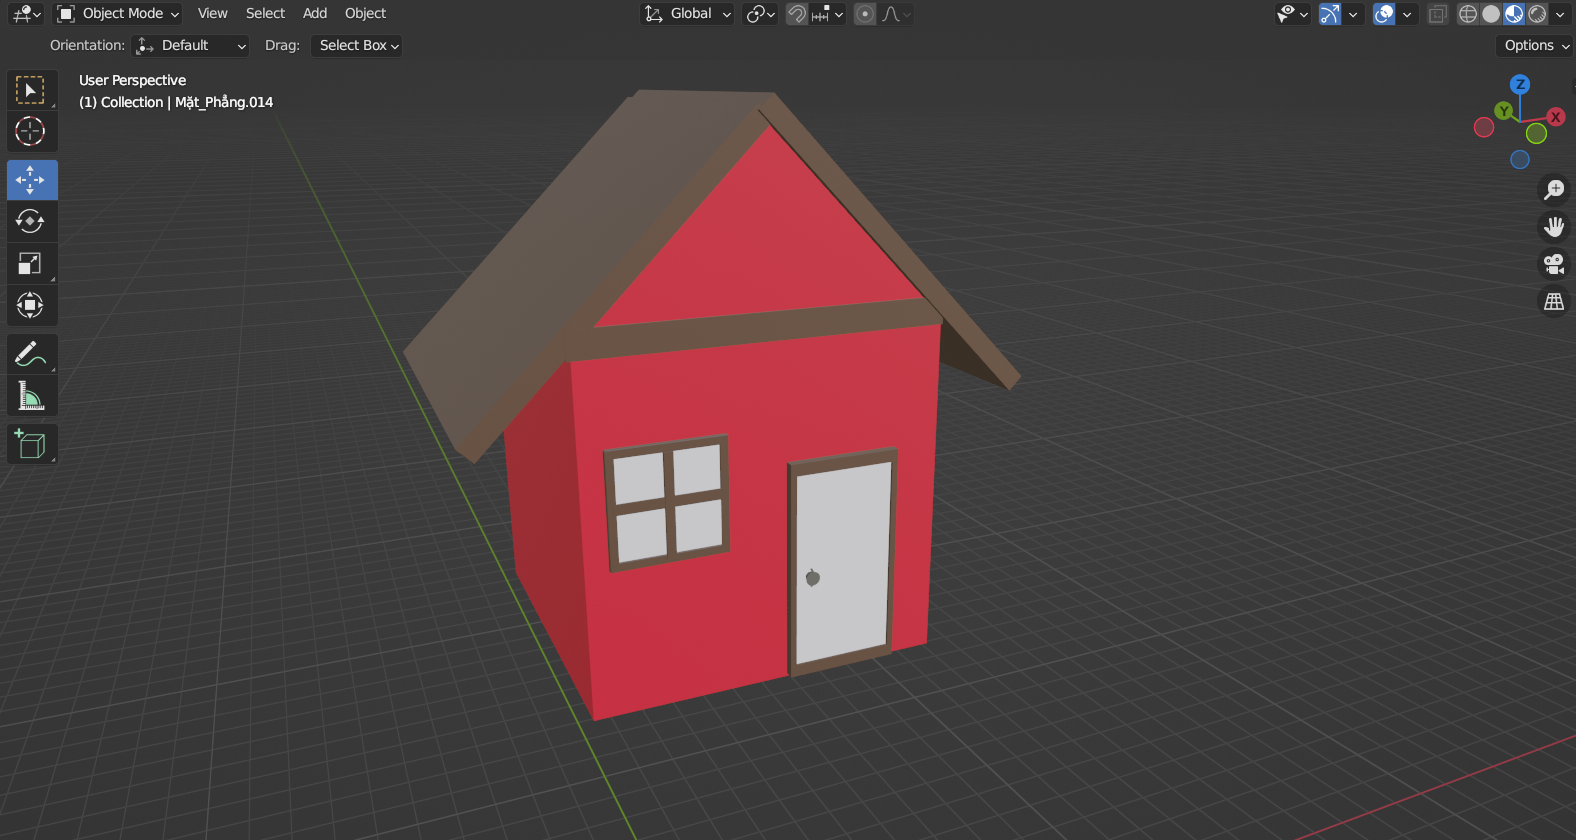
\includegraphics[scale = 0.4]{contents/house.png}
        \caption{Model bên ngoài ngôi nhà dựng bằng Blender}
    \end{figure}
\end{center}
\subsection{Chi tiết bên trong ngôi nhà}
\begin{center}
    \begin{figure}[!h]
        \centering
        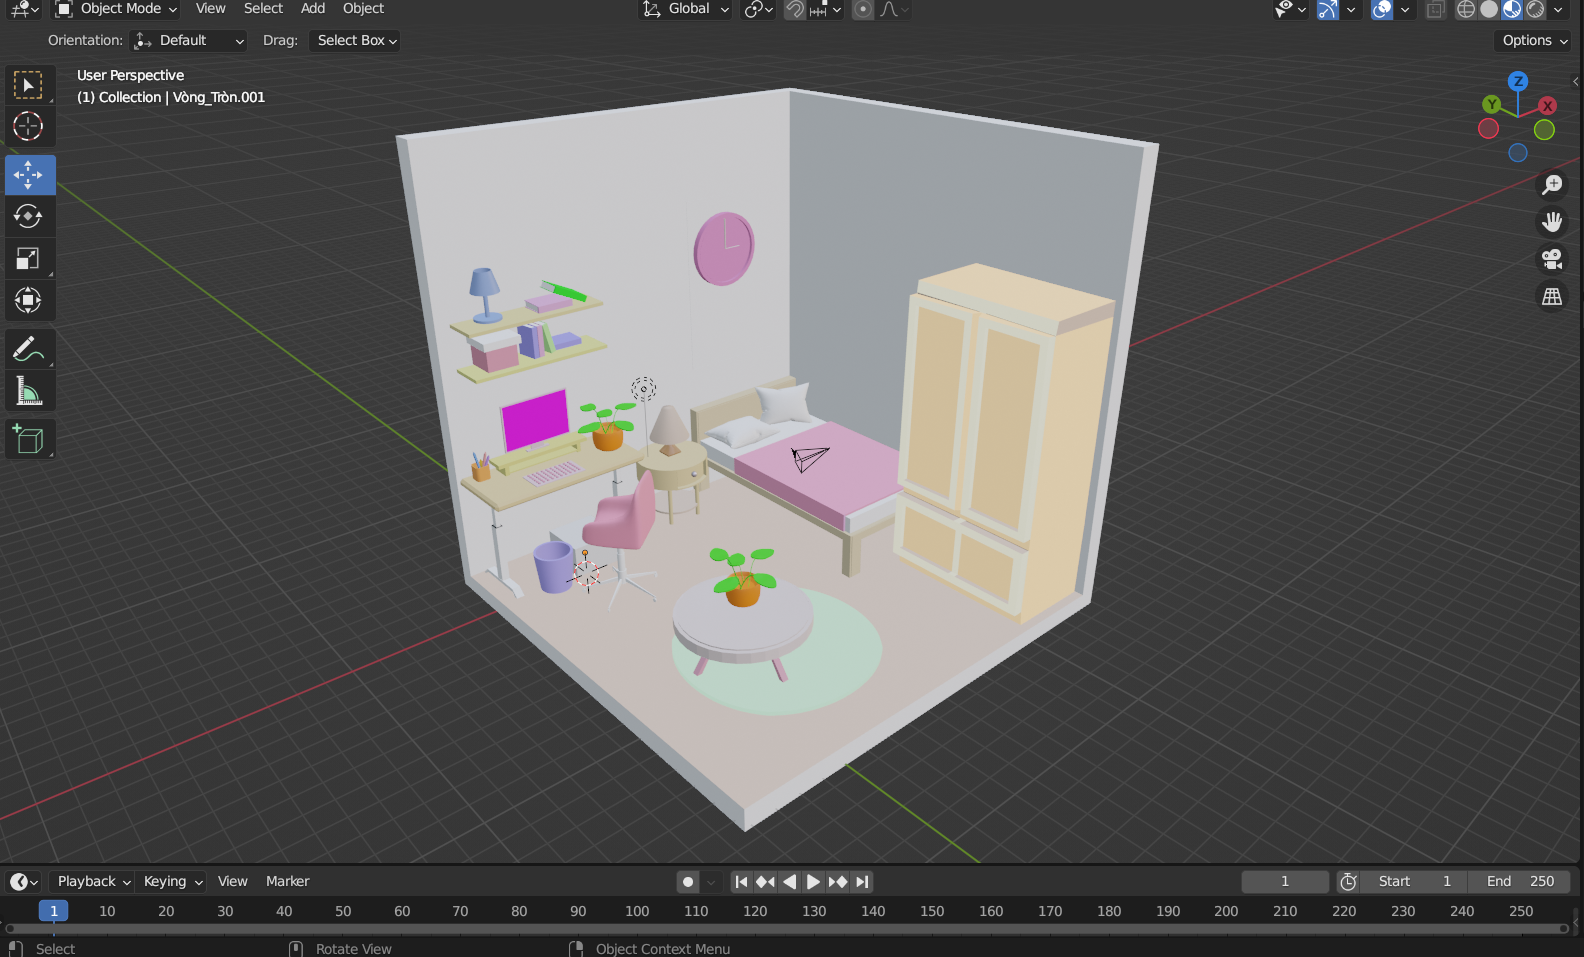
\includegraphics[scale = 0.35]{contents/fullhouse.png}
        \caption{Model chi tiết trong nhà dựng bằng Blender}
    \end{figure}
\end{center}

\newpage
\subsection{Cây}
\begin{center}
    \begin{figure}[!h]
        \centering
        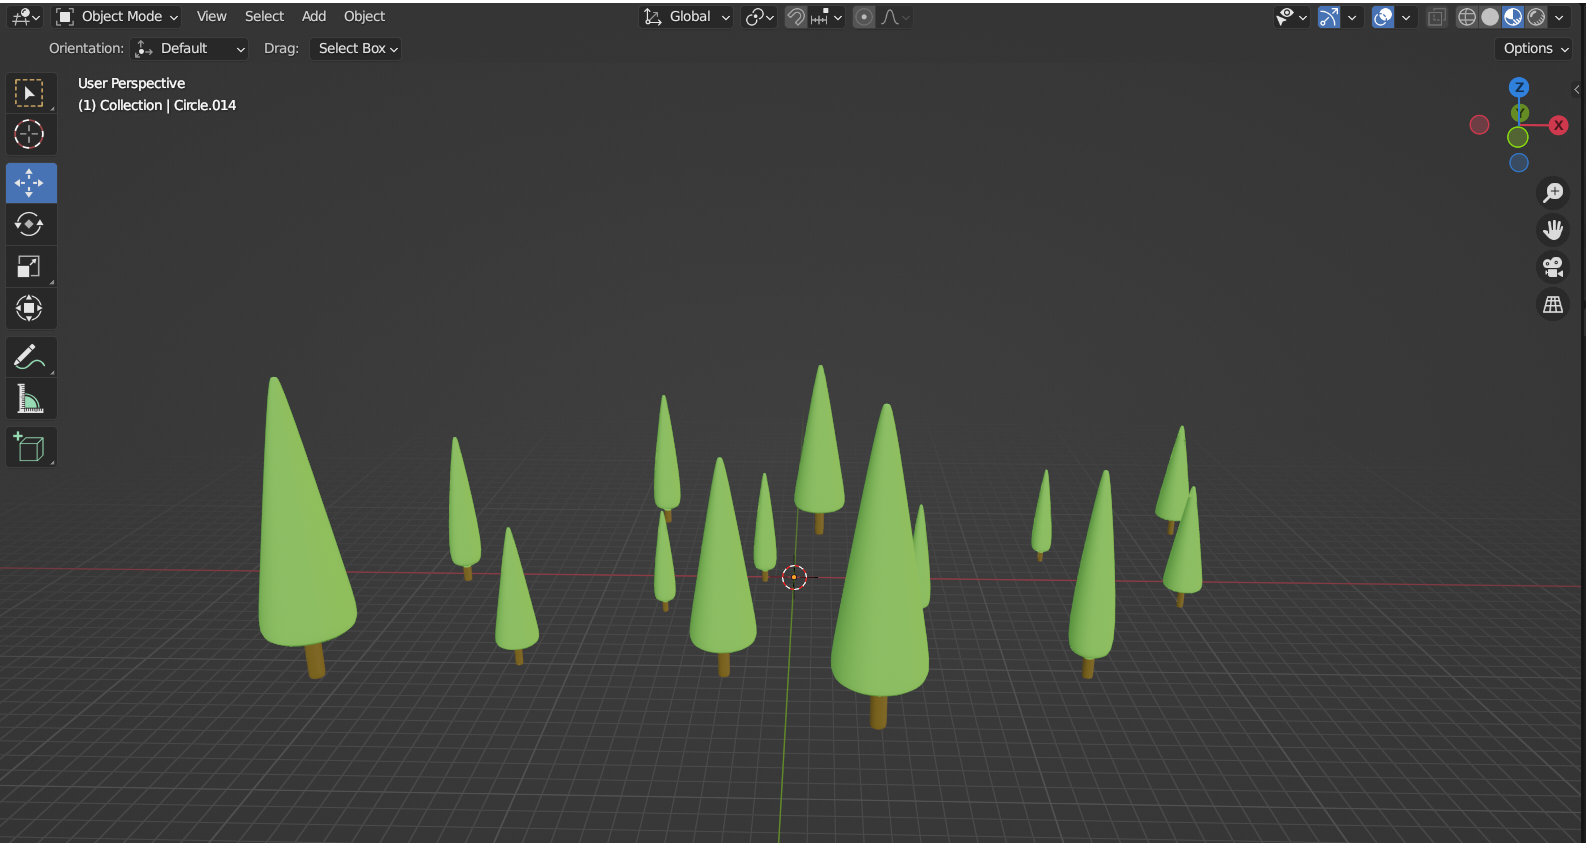
\includegraphics[scale = 0.35]{contents/tree.png}
        \caption{Model rừng cây dựng bằng Blender}
    \end{figure}
\end{center}


\subsection{Mây}
\begin{center}
    \begin{figure}[!h]
        \centering
        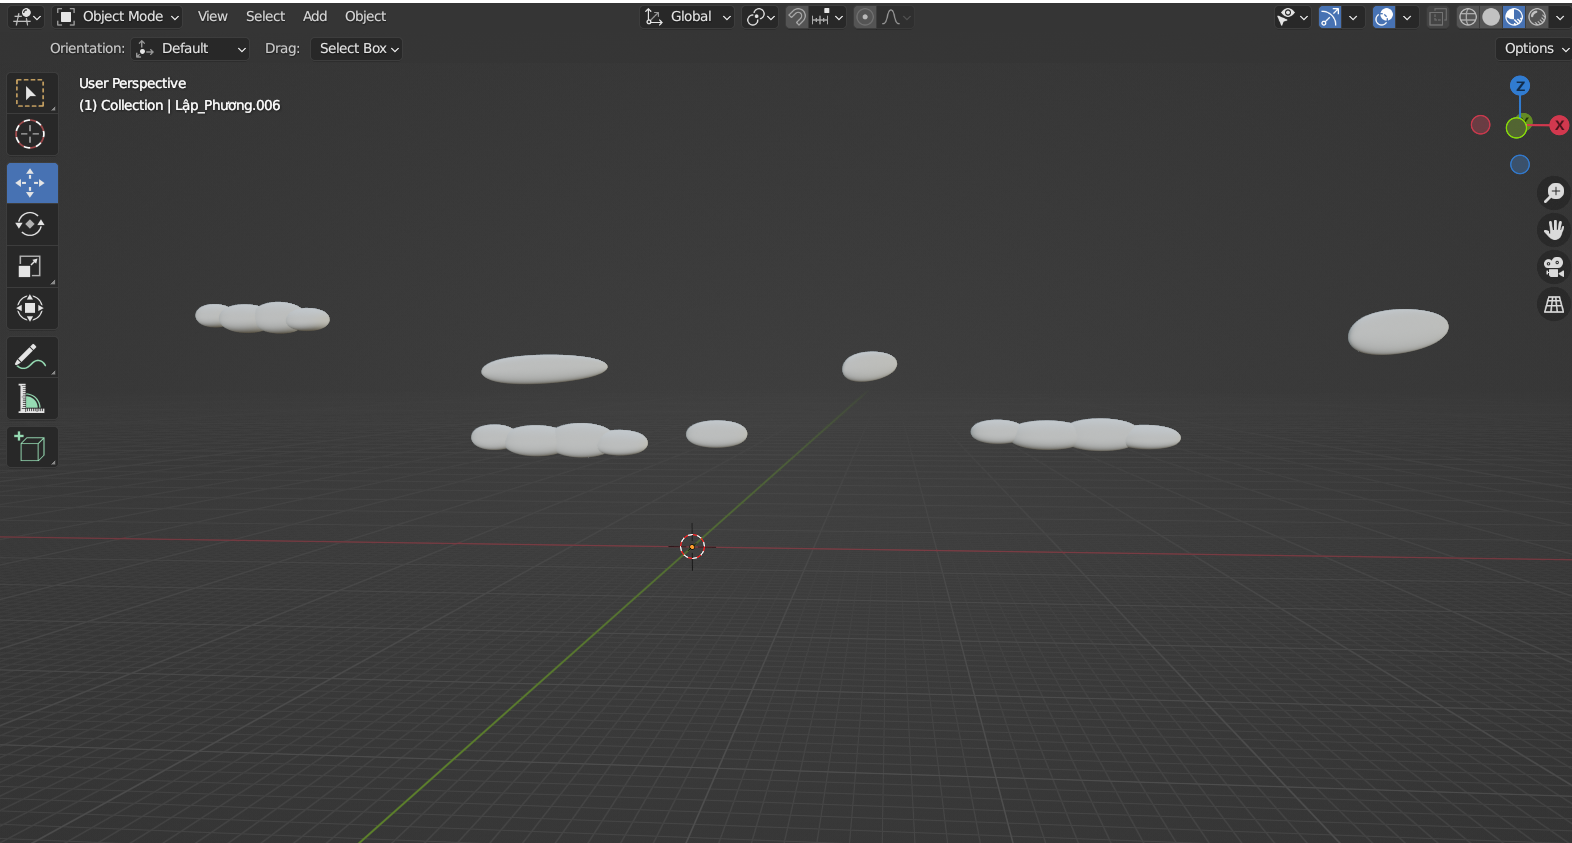
\includegraphics[scale = 0.35]{contents/cloud.png}
        \caption{Model các đám mây dựng bằng Blender}
    \end{figure}
\end{center}
\newpage
\section{Các objects khác}
\subsection{Nền trời}
Được tạo nên từ mặt bên trong của hình cầu với vật liệu là MeshPhongMaterial:
\begin{itemize}
    \item map: sử dụng texture nền bầu trời
    \item side:THREE.DoubleSide,
    \item shadowSide:THREE.DoubleSide 
\end{itemize}

\subsection{Nền đất}
Được tạo nên từ bề mặt bên ngoài của hình cầu với vật liệu là MeshStandardMaterial:
\begin{itemize}
    \item map: sử dụng texture nền thảm cỏ
    \item side:THREE.FrontSide
    \item transparent: false
    \item metalness:0
\end{itemize}

\begin{center}
    \begin{figure}[!h]
        \centering
        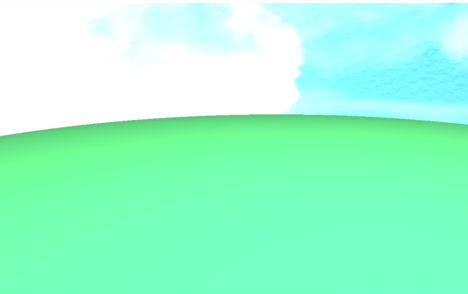
\includegraphics[scale = 1]{contents/day.png}
        \caption{Khung cảnh ngoài trời tạo bởi nền trời và đất}
    \end{figure}
\end{center}

\begin{center}
    \begin{figure}[!h]
        \centering
        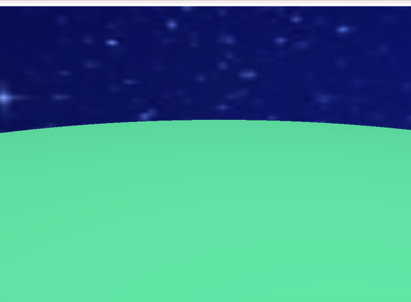
\includegraphics[scale = 1]{contents/night.png}
        \caption{Khung cảnh ngoài trời tạo bơi nền trời và đất}
    \end{figure}
\end{center}

\subsection{Hòn đá}
Được tạo nên từ hình cầu với vật liệu là MeshLambertMaterial:
\begin{itemize}
    \item color:"\#a0a0a0", 
     \item     side:THREE.DoubleSide,
    \item         shadowSide:THREE.DoubleSide
\end{itemize}


\subsection{Khung nhà}
Với khung cảnh trong nhà, do model được đọc vào chỉ là 1 góc nên để tạo độ chân thật cho khung cảnh này thì ở đây có vẽ thêm 1 cái hình hộp.\\

Hình hộp này có vật liệu là MeshLambertMaterial:
\begin{itemize}
    \item side:THREE.DoubleSide,
    \item shadowSide:THREE.DoubleSide
\end{itemize}

\newpage
\section{kỹ thuật sử dụng}
Sử dụng thư viện \textbf{dat.gui.js} để thay đổi khung cảnh xung quanh
\subsection{Điều chỉnh khung hình}
Sản phẩm này gồm có 2 khung cảnh :
\begin{itemize}
    \item Ngoài trời
    \item Trong nhà
\end{itemize}
Vì thế khi thay đổi cảnh thì cần phải set lại camera.
\begin{lstlisting}[language = java]
 gui.add(controls, "switchCamera", {"out":0, "in":1}).onChange(function(e){
            switch (parseInt(e)){
                case 0: 
                    cam.position.set(0, 20, 110);
                    //cam.lookAt(scene.position);
                    break;
                case 1: 
                    cam.reset();
                    cam = cam1;
                    //cam.lookAt(scene1.position);
                    break;
            }
        });
\end{lstlisting}

Để dễ hơn trong việc lập trình, ở đây có sử dụng 2 camera và 2 scene khác nhau nên việc điều chỉnh camera ảnh hưởng đến scene. Khi đó ta cũng cần cập nhật lại scene ở phần \textbf{myRender} như sau:
\begin{lstlisting}[language = java]
if (controls.switchCamera == 0){
            renderer.render(scene, cam);
        }else{
            renderer.render(scene1, cam1);
        } 
\end{lstlisting}

Lúc này ta có thể lựa dễ dàng chọn khung hình mà mình muốn.

\subsection{Điều chỉnh background}
Với khung cảnh ngoài trời thì sẽ có 2 lựa chọn là ban ngày hoặc ban đêm vì thế nếu muốn thay đổi chúng ta cần:
\begin{itemize}
    \item Thay đổi texture của nền trời
    \item Thay đổi các loại màu đèn 
\end{itemize}
\begin{lstlisting}[language = java]
 gui.add(controls, "display", {"bright":0, "dark":1}).setValue(0).onChange(function(e){
            switch (parseInt(e)){
                case 0:
                    url_troi = textureLoader.load("btl/sky4.jpg");
                    sphereMat1.map = url_troi;
                    scene.remove(pointLight_dark);
                    scene.remove(ambientLight_dark);
                    scene.add(ambientLight);
                    scene.add(pointLight); 
                    break;
                case 1: 
                    url_troi = textureLoader.load("btl/star1.jpg");
                    sphereMat1.map = url_troi;
                    scene.remove(pointLight);
                    scene.remove(ambientLight);
                    scene.add(ambientLight_dark);
                    scene.add(pointLight_dark);
                    break;
            }
        });
\end{lstlisting}

\newpage
\section{Hướng phát triển sản phẩm}
Với mong muốn hoàn thiện sản phẩm này tốt hơn nữa thì nhóm chúng em có đề ra một số bước phát triển thêm như sau:
\begin{itemize}
    \item Liên kết 2 khung cảnh với nhau thông qua việc ấn vào cánh cửa của ngôi nhà
    \item Cải thiện phần khung nhà ở phần trong nhà tương ứng với ngôi nhà bên ngoài hơn.
    \item Thiết kế giao diện đẹp mắt hơn
    \item ...

\end{itemize}
\newpage
\input{contents/Chapter cuối}


\end{document} 
